\documentclass[a4paper,10pt,DIV=14]{scrartcl}
\usepackage{graphicx}
\usepackage[utf8]{inputenc} % korrekte Darstellung von Umlauten u. Sonderzeichen
\usepackage[ngerman]{babel} % Sprachpaket, ngerman = neue deutsche Rechtschreibung
\usepackage{amsmath} % Setzen mathematischer Formeln
\usepackage{titlesec}
\usepackage{float}
\usepackage{caption}
\usepackage{fancyvrb}
\usepackage{siunitx}
\usepackage{booktabs}
\usepackage{enumitem}

\usepackage{tabularx}
\newcolumntype{L}[1]{>{\raggedright\arraybackslash}p{#1}} % linksbündig mit Breitenangabe
\newcolumntype{C}[1]{>{\centering\arraybackslash}p{#1}} % zentriert mit Breitenangabe
\newcolumntype{R}[1]{>{\raggedleft\arraybackslash}p{#1}} % rechtsbündig mit Breitenangabe

\newcommand{\gqq}[1]{\glqq{}#1\grqq{}}
\newcommand{\gq}[1]{\glq{}#1\grq{}}
\newcommand{\dg}[1]{#1^\circ}

\renewcommand{\thesection}{Aufgabe \arabic{section}:}
\renewcommand{\thesubsection}{\alph{subsection})}
\titleformat*{\subsection}{\normalfont\fontfamily{phv}\fontsize{12}{15}\selectfont}


\captionsetup[figure]{labelformat=empty}


\begin{document}

\title{Graphische Datenverarbeitung WS17/18 \\ Theorieübung 1}
\author{
  Salmah Ahmad (2880011)
  \and
  Markus Höhn (1683303)
  \and
  Tobias Mertz (2274355)
  \and
  Steven Lamarr Reynolds (1620638)
  \and
  Sascha Zenglein (2487032)
}

\maketitle

\section{Pipeline}

\subsection{Aus was besteht der Input der Pipeline?}
Der Input der Pipeline besteht aus einer gegebenen Szenenbeschreibung.


\subsection{Zum Input gehören unter anderem \gqq{Objekte}. In welcher Form sind konkrete \gqq{Objekte} im Input gegeben?}

\begin{itemize}[itemsep=0pt]
	\item (virtuelle) Kamera
	\item Dreidimensionale Objekte
	\item Lichtquellen
	\item Beleuchtungsalgorithmen
	\item Texturen
	\item ...
\end{itemize}


\subsection{Was ist der Output der Pipeline?}
Der Output der Pipeline ist ein 2D Bild der gegeben Szenenbeschreibung.


\subsection{Weshalb ist eine Pipeline die aus $n$ Abschnitten besteht (theoretisch) $n$-mal schneller als eine Pipeline mit nur einem Abschnitt?}
Bei einer Pipeline mit $n$ Abschnitten kann eine parallele Verarbeitung durchgeführt werden.


\subsection{Weshalb ist die Pipeline Geschwindigkeit vom Bottleneck abhängig? Wieso warten die anderen Pipeline-Abschnitte bis der Bottleneck-Abschnitt fertig ist?}
Der Bottleneck-Abschnitt ist der langsamste der Pipeline. Die Berechnung eines Frames basiert auf den Ergebnissen der vorausgegangenen Pipeline-Abschnitte. Daher ist die Geschwindigkeit der Pipeline abhängig vom langsamsten Verarbeitungsschritt.


\section{Model \& View Transformation}

\subsection{Stellen Sie die Gleichung $(x, z)^T = f(u,v)$ auf, die die $u, v$ Koordinaten in das Weltkoordinatensystem transformiert. Bestimmen Sie nun die Position der Szenenobjekte bezüglich des Weltkoordinatensystems.}

$$f(u,v) = \begin{pmatrix}
\cos(\alpha) & \sin(\alpha)  & r \cdot \cos(\alpha)  \\
\sin(\alpha) & -\cos(\alpha) & -r \cdot \sin(\alpha) \\
0            & 0             & 1                     \\
\end{pmatrix} \cdot \begin{pmatrix} u \\ v \\ 1 \\ \end{pmatrix} $$

Ergebnisse:
\begin{itemize}[itemsep=0pt]
	\item Sonne: $ (0, 0)^T $
	\item Planet: $ (-2\sqrt{3}, -2)^T $
	\item Mond: $ (2 - 2\sqrt{3}, -3)^T $
\end{itemize}


\subsection{Bestimmen Sie, welche Translation und welche Rotation auf die Szene ausgeübt werden müssen, um die Kamera in den Ursprung zu verschieben und anschließend die Blickrichtung nach -z zu rotieren.}

\begin{itemize}
	\item Translation: $ (-2, -2\sqrt{3})^T $
	\item Winkel: $ \arctan(\frac{2}{2\sqrt{3}}) = \dg{30} $
	\item Rotation: $ \begin{pmatrix}	\cos(\dg{30}) & -\sin(\dg{30}) \\ \sin(\dg{30}) & cos(\dg{30}) \\ \end{pmatrix}
	= \begin{pmatrix} \frac{\sqrt{3}}{2} & \frac{1}{2} \\ \frac{1}{2} & \frac{\sqrt{3}}{2} \end{pmatrix} $
\end{itemize}


\subsection{Berechnen Sie die Position der Szenenobjekte nach der Model- und View-Transformation. Fertigen Sie eine Skizze an.}



\section{Optische Triangulation}

\subsection{Stellen Sie die Gleichung $\beta = f_1(p)$ auf, um aus einer Pixelposition $p$ den Winkel $\beta$ zu berechnen. Verwenden Sie dabei die Koordinate des Pixelmittelpunktes! \\ Wie groß ist $\beta$, wenn der Laserpunkt in der Mitte von Pixel 5223 registriert wird?}


$$f_1(p) = \arctan \left( \frac{\vert (\frac{p_x}{8191}) \cdot 48mm - 24mm) \vert}{24 mm} \right) := \beta $$

$f_1(5223) = \dg{15,38}$

\subsection{Stellen Sie die Gleichung $\alpha = f_2(\gamma)$ auf, um aus dem Spiegelwinkel $\gamma$ den Winkel $\alpha$ zu berechnen. \\ Berechnen Sie $f_2(45^\circ)$ und $f_2(77^\circ)$.}


\begin{figure}[h]
	\begin{minipage}[c]{0.49\textwidth}
		\centering						
		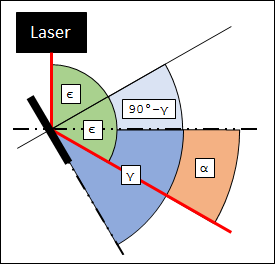
\includegraphics[width=.95\linewidth]{alpha.png}
	\end{minipage}
	\hfill
	\begin{minipage}[c]{0.49\textwidth}
		\centering
		$ \begin{aligned}
			\alpha & = \epsilon - (\dg{90} - \gamma) \qquad \textit{mit} \quad \epsilon = \dg{90} - (\dg{90} - \gamma) \\
			       & = (\dg{90} - (\dg{90} - \gamma)) - (\dg{90} - \gamma) \\
		           & = \dg{90} - \dg{90} + \gamma - \dg{90} + \gamma \\
		           & = 2\gamma - \dg{90}
		\end{aligned} $
	\end{minipage}
	\caption*{b) Berechnung $\alpha$}
\end{figure}

\begin{itemize}[itemsep=0pt]
	\item $f_2(\dg{45}) = 2 \cdot \dg{45} - \dg{90} =  \dg{0}$
	\item $f_2(\dg{77}) = 2 \cdot \dg{77} - \dg{90} =  \dg{64}$
\end{itemize}


\subsection{Stellen Sie die Gleichung $z = f_3(\alpha, \beta)$ auf, um aus den Winkeln $\alpha$ und $\beta$ den Tiefenwert $z$ zu berechnen. \\ Welcher Tiefenwert gehört zu den Winkeln $\alpha = 15^\circ$ und $\beta = 30^\circ$?}

\begin{figure}[!htbp]
	\centering
	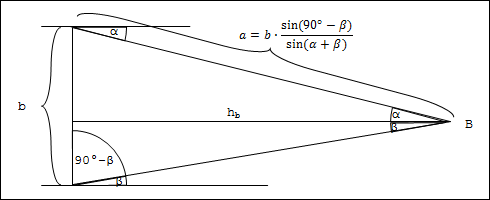
\includegraphics[width=.95\linewidth]{z.png}
	\caption*{c) Berechnung $z$}
\end{figure}

Mithilfe des Sinussatzes gilt: $$ a = b \cdot \frac{\sin(\dg{90} - \beta)}{\sin(\alpha + \beta)} $$
Weiter gilt: $$ \cos(\alpha) = \frac{h_b}{a} $$
Mit $h_b := z$ gilt:
$$ z = \cos(\alpha) \cdot \frac{b \cdot \sin(\dg{90} - \beta)}{\sin(\alpha + \beta)} $$

Für $\alpha = \dg{15}$ und $\beta = \dg{30}$ folgt:
$$ z = \cos(\dg{15}) \cdot \frac{150mm \cdot \sin(\dg{90} - \dg{30})}{\sin(\dg{15} + \dg{30})} = 177.5mm $$

\subsection{Stellen Sie die Gleichung $x = f_4(\beta, z)$ auf, um aus dem Winkel $\beta$ und $z$ die $x$-Koordinate zu berechnen \\ Berechnen sie $f_4(40^\circ, 100cm)$.}

\subsection{Stellen Sie nun die Gesamtgleichung $(x,z)^T = f_5(p, \gamma)$ auf, um aus der Pixelposition $p$ und dem Winkel $\gamma$ die Koordinaten $(x, z)^T$ des abgetasteten Punktes zu berechnen.}

\subsection{Zum Spiegelwinkel $\gamma = 67^\circ$ wird ein Laserpunkt im Mittelpunkt von Pixel 5730 registriert. Welche Koordinaten hat der abgetastete Punkt mit oben beschriebenen Aufbau?}

\end{document}
